\documentclass[12pt]{article}
\usepackage[total={6in, 10in}]{geometry}

%langue
\usepackage[T1, T2A]{fontenc}
\usepackage[utf8]{inputenc}
\usepackage[english, ukrainian]{babel}


\author{студент: Недождій Олексій Сергійович \\
         викладач: Гордійко Наталія Олександрівна}
\title{Лабораторна робота № 6.2\\
    З методiв аналiзу та обробки\\
    експериментальних даних\\
       Варіант №16}
\date{}

\usepackage{lmodern}
\usepackage{graphicx}
\usepackage{color}
\usepackage{listings}
\usepackage{hyperref}
\usepackage{amsmath}
\usepackage{amsfonts}
\usepackage{epstopdf}
\usepackage{matlab}

\sloppy
\epstopdfsetup{outdir=./}
\graphicspath{ {./lab6_2_images/} }

\begin{document}
\maketitle

\section{Завдання}
\begin{enumerate}
    \item
        За допомогою мікрофону ввести у комп'ютер аудіосигнал (назвіть свої
        прізвище, ім’я та групу). Відтворити (прослухайте) введену інформацію.
    \item
        Змінити частоту дискретизації fs для пришвидшення та уповільнення
        відтворення запису та відтворити отримані сигнали.
    \item
        Записати введене аудіо у вигляді wav-файлу та mat-файлу. Вивести
        інформацію про отриманий wav-файл.
    \item
        Побудувати графік сигналу та його спектрограму, а також
        амплітудний та фазовий спектри.I
    \item
        Завантажити файл сигналу у Signal Analyzer Toolbox та на його
        прикладі дослідити можливості даного Toolbox, зокрема, отримати відповідні
        графіки, спектрограми тощо.
\end{enumerate}

\newpage
\section{Рішення}
\subsection*{Записуєм данні в файл}
\begin{par}
\begin{flushleft}
Задаєм константы t та Fs
\end{flushleft}
\end{par}

\begin{matlabcode}
t = 5;
Fs = 8000;
nBits = 16;
nChannels = 1;
deviceId = 1;
\end{matlabcode}

\begin{par}
\begin{flushleft}
Записуєм аудіо
\end{flushleft}
\end{par}

\begin{matlabcode}
disp("Start recording");
\end{matlabcode}
\begin{matlabcode}
audio = audiorecorder(Fs, nBits, nChannels, deviceId);
recordblocking(audio, t)
disp("End recording")
\end{matlabcode}

\begin{par}
\begin{flushleft}
Виводим аудіо
\end{flushleft}
\end{par}

\begin{matlabcode}
play(audio);
\end{matlabcode}

\begin{par}
\begin{flushleft}
Записуєм аудіо до файлу
\end{flushleft}
\end{par}

\begin{matlabcode}
audio_data = getaudiodata(audio);
audiowrite('audio.wav', audio_data, Fs);
save('audio.mat', 'audio_data', 'Fs');
\end{matlabcode}





\begin{par}
\begin{flushleft}
Інформація про файл
\end{flushleft}
\end{par}

\begin{matlabcode}
info = audioinfo('audio.wav');
disp(info);
\end{matlabcode}
\begin{matlaboutput}
             Filename: 'D:\university\5\ma_labs\ma_lab6\audio.wav'
    CompressionMethod: 'Uncompressed'
          NumChannels: 1
           SampleRate: 8000
         TotalSamples: 40000
             Duration: 5
                Title: []
              Comment: []
               Artist: []
        BitsPerSample: 16
\end{matlaboutput}

\begin{par}
\begin{flushleft}
Зчитуєм аудіо з файлу
\end{flushleft}
\end{par}

\begin{matlabcode}
[audio, Fs] = audioread('audio.wav');
t = length(audio) / Fs; %time
\end{matlabcode}

\begin{par}
\begin{flushleft}
Оригінаьне аудіо
\end{flushleft}
\end{par}

\begin{matlabcode}
sound(audio, Fs);
pause(t)
\end{matlabcode}

\begin{par}
\begin{flushleft}
Прискорене аудіо
\end{flushleft}
\end{par}

\begin{matlabcode}
sound(audio, Fs * 2);
pause(t / 2)
\end{matlabcode}

\begin{par}
\begin{flushleft}
Уповільнене аудіо
\end{flushleft}
\end{par}

\begin{matlabcode}
sound(audio, Fs / 2);
\end{matlabcode}

\vspace{1em}

\begin{par}
\begin{flushleft}
Графік сигналу
\end{flushleft}
\end{par}

\begin{matlabcode}
plot(audio);
title("Signal graph");
grid on;
\end{matlabcode}
\begin{center}
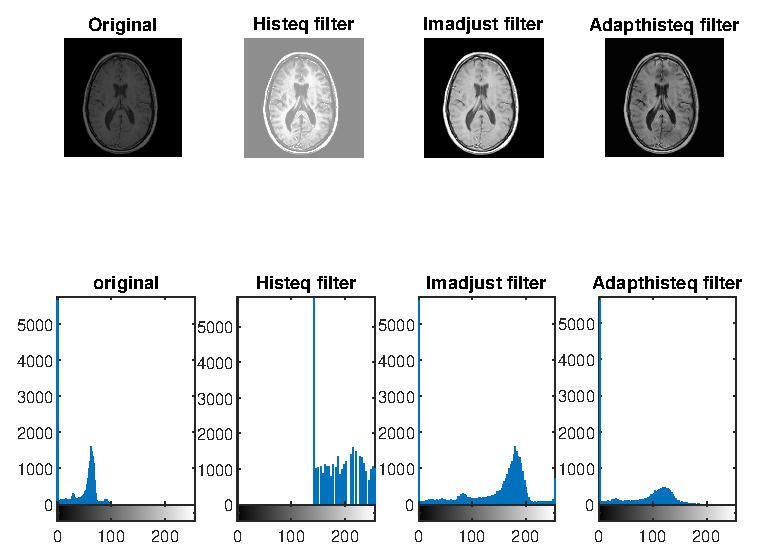
\includegraphics[width=\maxwidth{56.196688409433015em}]{figure_0}
\end{center}

\begin{par}
\begin{flushleft}
Спектрограма
\end{flushleft}
\end{par}

\begin{matlabcode}
spectrogram(audio, 256, 128, [], Fs, 'yaxis');
title('Spectrogram');
\end{matlabcode}
\begin{center}
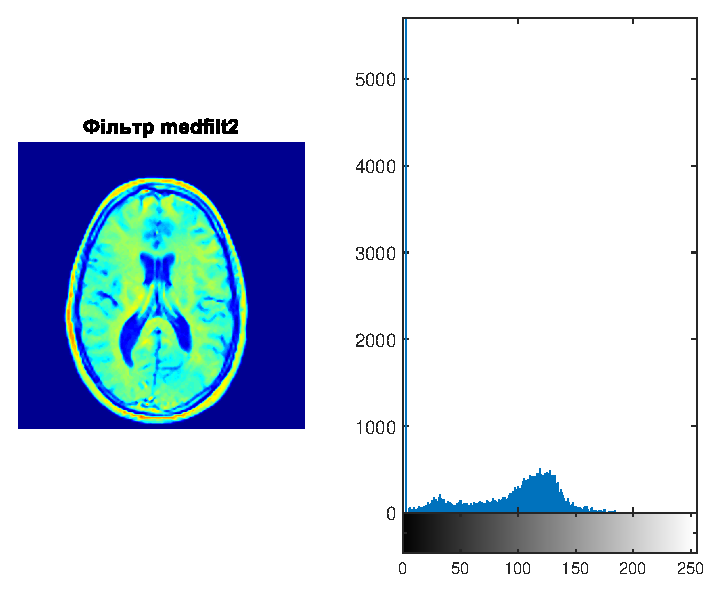
\includegraphics[width=\maxwidth{56.196688409433015em}]{figure_1}
\end{center}

\begin{par}
\begin{flushleft}
Амплітудний спектр
\end{flushleft}
\end{par}

\begin{matlabcode}
aspec = abs(fft(audio));
aspec = aspec(1 : end / 2);
afreq = (Fs / 2) * (1:length(aspec)) / length(aspec);
plot(afreq, aspec, 'k');
xlabel ('Frequency: Hz'); ylabel ('Amplitude spectrum');
grid on;
\end{matlabcode}
    \begin{center}
    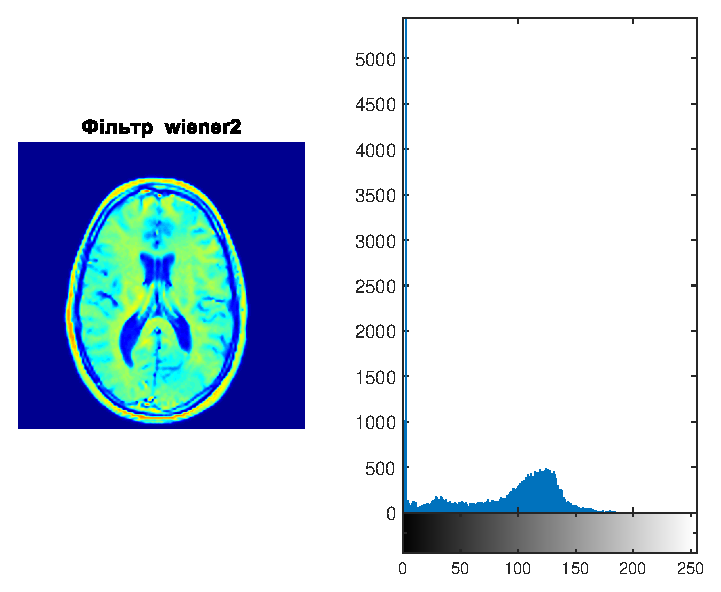
\includegraphics[width=\maxwidth{56.196688409433015em}]{figure_2}
    \end{center}

    \begin{par}
    \begin{flushleft}
    Фазовий спектр
    \end{flushleft}
    \end{par}

    \begin{matlabcode}
    fspec = phase (fft(audio));
    fspec = fspec (1:end/2);
    ffreq = (Fs / 2) * (1:length(fspec)) / length(fspec);
    plot(ffreq, fspec, 'k');
    xlabel ('Frequency: Hz'); ylabel ('Phase spectrum');
grid on;
\end{matlabcode}
\begin{center}
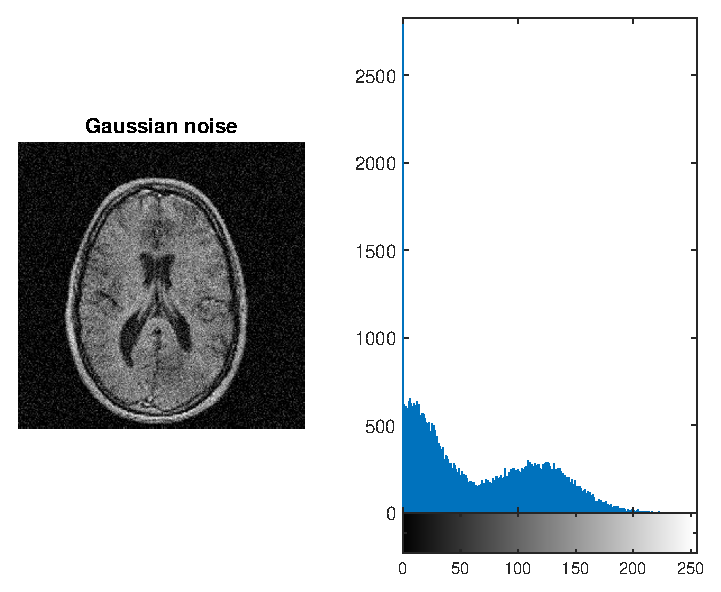
\includegraphics[width=\maxwidth{56.196688409433015em}]{figure_3}
\end{center}

\subsection*{Signal Analyzer ToolBox}
\begin{center}
    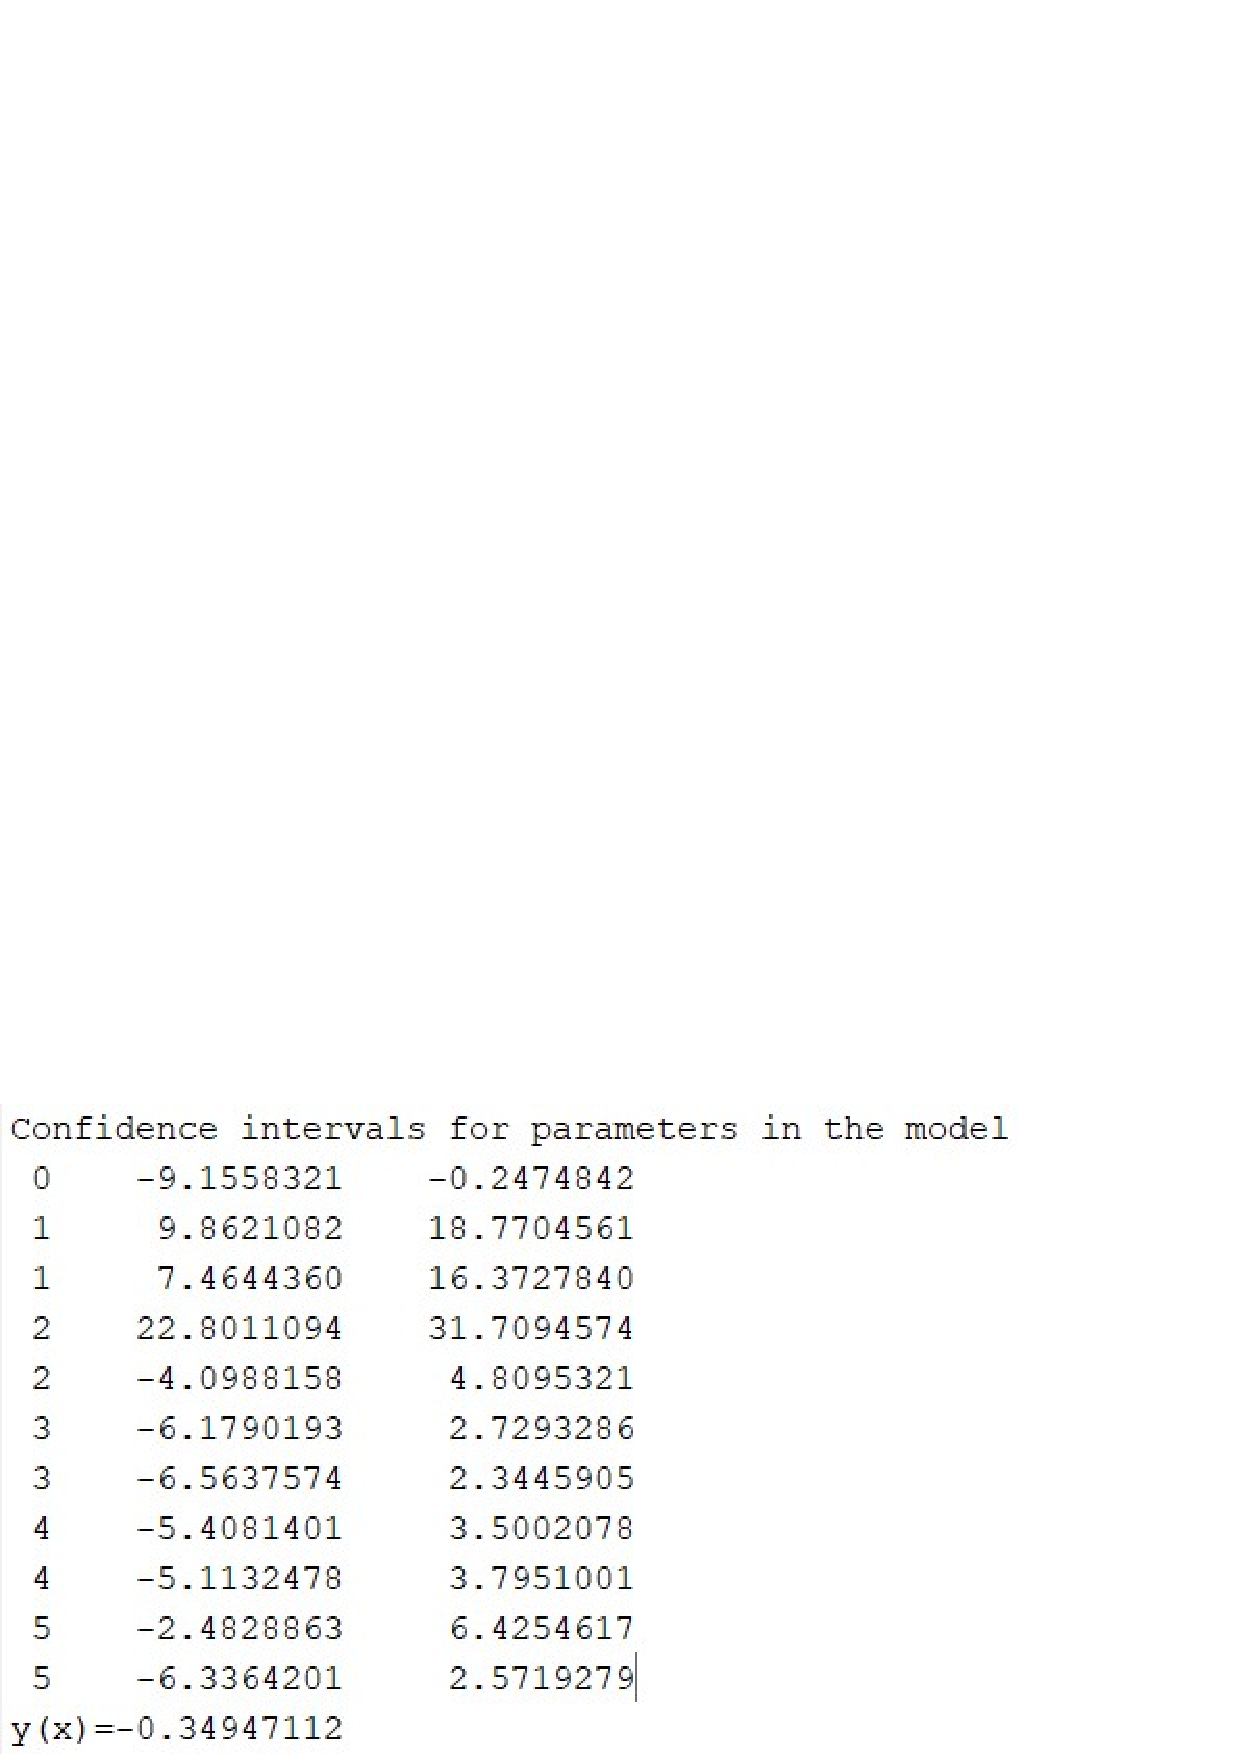
\includegraphics[scale=0.5]{Screenshot_1.jpg}
\end{center}
(Сигнал для тулбоксу інший, випадково перезаписався)

\section{Висновок}
Signal Analyzer ToolBox досить зручний щоб зробити швидко щось нескладне.
Але на мою думку для більш глубокого аналізу слід самому писати код.

\end{document}
